\documentclass{article}

\usepackage{amsmath}
\usepackage{amssymb}
\usepackage{enumerate}
\usepackage[spanish]{babel}
\usepackage{cancel}
\usepackage{caption}
\usepackage[margin=1.5in]{geometry}
\usepackage{graphicx}
\usepackage[utf8]{inputenc}
\usepackage{tcolorbox}
\usepackage{esint}
\usepackage{hyperref}
\hypersetup{
    colorlinks,
    citecolor=black,
    filecolor=black,
    linkcolor=black,
    urlcolor=black,
}

\renewcommand{\Bbb}{\mathbb}

\tcbuselibrary{theorems}

\title{Ejercicios de Análisis Matemático II A (63.01) \\
Guía 3 - Diferenciabilidad, tangentes \\
Cátedra Acero \\
1° C 2004}
\author{Darío Eduardo Ramos}

\begin{document}
\maketitle

\tableofcontents{}
\newpage

\section*{3.1}
\label{sec:3.1}
\addcontentsline{toc}{section}{\nameref{sec:3.1}}

\textbf{En los siguientes casos:} 

\begin{enumerate}
\bfseries

\item Calcular el gradiente de $f$ en el punto $P_0 = (x_0, y_0)$
\item En un gráfico en 3D, trazar aproximadamente la curva de nivel $C$ de $f$ que pasa por $P_0$, su recta tangente en $P_0$ y el gradiente de $f$ con origen en $P_0$.
\item (En el mismo gráfico) Ubicar el punto $Q_0$ de la superficie $z = f(x,y)$ cuya proyección en el plano $xy$ es $P_0$; dibujar aproximadamente la superficie $z$ en la vecindad de $Q_0$ y su plano tangente.
\item (En el mismo gráfico) Marcar sobre la superficie $z$ la curva cuya proyección en el plano $xy$ es $C$.
\item (En el mismo gráfico) Graficar el vector $N = (f'_x(P_0), f'_y(P_0), -1)$ con origen en $Q_0$.
\item ¿Qué relación hay entre los distintos objetos geométricos del gráfico? Explicar las relaciones con palabras y ponerlas en evidencia en los dibujos.

\end{enumerate}

\begin{enumerate}[(a)]
\bfseries

\item $f(x,y)=x^2+y^2, P_0 = (1,1)$
\item $f(x,y)=\sqrt{4-x^2-y^2}, P_0 = (1,-1)$
\item $f(x,y)=5+2x-3y, P_0=(0,0)$
\item $f(x,y)=7+xy, P_0=(0,0)$
\item $f(x,y)=7+x^2-y^2, P_0=(1,1)$
\item $f(x,y)=\sqrt{x^2+y^2/4}, P_0=(0,2)$

\end{enumerate}
\hrule

\subsection*{3.1.a}
\label{subsec:3.1.a}
\addcontentsline{toc}{subsection}{\nameref{subsec:3.1.a}}

\subsubsection*{3.1.a.1}
\label{subsubsec:3.1.a.1}
\addcontentsline{toc}{subsubsection}{\nameref{subsubsec:3.1.a.1}}

Por simple inspección, $f \in C^1$ y por ende existe el gradiente:

\begin{equation}
\overrightarrow{ \nabla f }(x,y) = (f_x(x,y), f_y(x,y)) = (2x, 2y)
\end{equation}

Ergo:

\begin{equation}
\tcboxmath[colback=orange!25!white,colframe=orange,title=3.1.a.1]
{
\overrightarrow{ \nabla f }(x_0,y_0) = (2, 2)
}
\end{equation}

\subsubsection*{3.1.a.2}
\label{subsubsec:3.1.a.2}
\addcontentsline{toc}{subsubsection}{\nameref{subsubsec:3.1.a.2}}

La curva de nivel $k$ de f es:

\begin{equation}
C_k(f) = \{ (x,y) \in \Bbb R^2 / x^2 + y^2 = k, k \in \Bbb R, k \geq 0 \}
\end{equation}

Por lo tanto, la curva de nivel asociada a $P_0$ es:

\begin{equation}
(x_0)^2 + (y_0)^2 = 2 \Rightarrow k = 2
\end{equation}

\begin{equation}
\tcboxmath[colback=orange!25!white,colframe=orange,title=3.1.a.2]
{
C_2(f) = \{ (x,y) \in \Bbb R^2 / x^2 + y^2 = 2 \}
}
\end{equation}

Para hallar la recta tangente a $C_2(f)$, conviene parametrizarla como curva en $\Bbb R^2$. Es un círculo de radio $\sqrt{2}$, por ende:

\begin{subequations}
\begin{align}
& C_2(f): \sigma(t) = (\sqrt{2} \cos(t), \sqrt{2} \sin(t)), t \in [0, 2\pi) \\
& \sigma'(t) = (-\sqrt{2} \sin(t), \sqrt{2} \cos(t))
\end{align}
\end{subequations}

Ahora bien, el punto donde se desea evaluar la recta tangente es $(x_0, y_0) = (1, 1)$. Sea $t_0$ el valor que hace $\sigma(t_0) = (x_0, y_0)$. El próximo paso es calcular ese valor.

\begin{equation}
(\sqrt{2} \cos(t_0), \sqrt{2} \sin(t_0)) = (1, 1) \Rightarrow t_0 = \frac{\pi}{4}
\end{equation}

El vector dirección de la recta tangente en $\sigma(t_0)$ es $\sigma'(t_0) = (-1, 1)$. La recta tangente en $(1, 1)$ es entonces:

\begin{equation}
\tcboxmath[colback=orange!25!white,colframe=orange,title=3.1.a.2]
{
L_T: (-1, 1) \alpha + (1, 1)
}
\end{equation}

Gráficamente, estos elementos pueden visualizarse en la figura \ref{fig:1-a-2}.

\begin{figure}[ht]
\caption{Curva de nivel, recta tangente y gradiente}
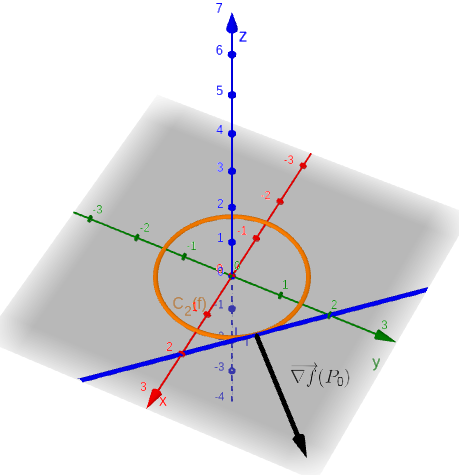
\includegraphics[scale=0.35]{img/ejercicios/3/1-a-2.png} 
\centering
\label{fig:1-a-2}
\end{figure}

Nótese que el gradiente, tomando como origen el vector $(x_0, y_0)$, es un vector ortogonal al vector dirección de la recta tangente.

\subsubsection*{3.1.a.3}
\label{subsubsec:3.1.a.3}
\addcontentsline{toc}{subsubsection}{\nameref{subsubsec:3.1.a.3}}

Primero, para calcular el plano tangente en un punto $P_0$, recúerdese que ello puede realizarse usando las derivadas parciales:

\begin{equation}
\Pi_T: z-z_0 - f_x(P_0) (x-x_0) - f_y(P_0) (y-y_0) = 0
\end{equation}

Para este caso, $x_0 = 1$, $y_0 = 1$, $z_0 = 2$, $f_x(x,y) = 2x$, y $f_y(x,y) = 2y$. Ergo:

\begin{subequations}
\begin{align}
& z-2 - 2 (x-1) - 2(y-1) = 0 \\
& z-2 -2x +2 -2y +2 = 0 \\
& -2x -2y + z + 2 = 0
\end{align}
\end{subequations}

\begin{equation}
\tcboxmath[colback=orange!25!white,colframe=orange,title=3.1.a.3]
{
\Pi_T: 2x + 2y -z -2 = 0
}
\end{equation}

La superficie asociada a $z = x^2 + y^2$ es un paraboloide centrado en el origen. El punto $Q_0$ no es otra cosa que $(x_0, y_0, f(x_0, y_0)) = (1, 1, 2)$. Agregando la superficie y el plano tangente al gráfico previo, se obtiene la figura \ref{fig:1-a-3}.

\begin{figure}[ht]
\caption{Superficie y plano tangente}
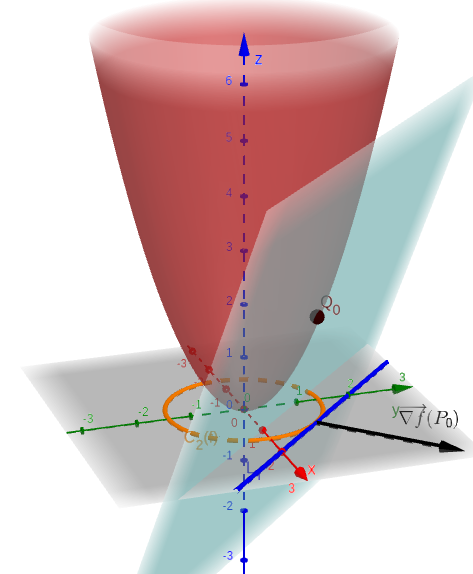
\includegraphics[scale=0.35]{img/ejercicios/3/1-a-3.png} 
\centering
\label{fig:1-a-3}
\end{figure}

\subsubsection*{3.1.a.4}
\label{subsubsec:3.1.a.4}
\addcontentsline{toc}{subsubsection}{\nameref{subsubsec:3.1.a.4}}

Recordando que las curvas de nivel pueden pensarse como cortes de la superficie a lo largo del eje $z$, la curva pedida es $C_2(f)$, extendida a $\Bbb R^3$ fijando la componente $z = 2$. En otras palabras, es un círculo de radio $\sqrt{2}$ centrado en el origen del plano $z = 2$. Ello puede visualizarse en color verde claro en la figura \ref{fig:1-a-4}.

\begin{figure}[ht]
\caption{Curva de nivel en superficie}
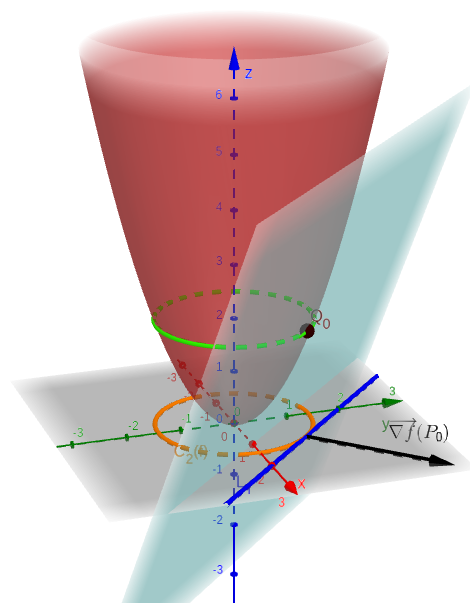
\includegraphics[scale=0.35]{img/ejercicios/3/1-a-4.png} 
\centering
\label{fig:1-a-4}
\end{figure}

\subsubsection*{3.1.a.5}
\label{subsubsec:3.1.a.5}
\addcontentsline{toc}{subsubsection}{\nameref{subsubsec:3.1.a.5}}

El valor de $N$ es:

\begin{equation}
N = (fx(x_0,y_0), f_y(x_0,y_0), -1) = (2, 2, -1)
\end{equation}

Graficando $N$ con origen en $Q_0$, se obtiene el vector negro de la figura \ref{fig:1-a-5}.

\begin{figure}[ht]
\caption{Vector normal a la superficie}
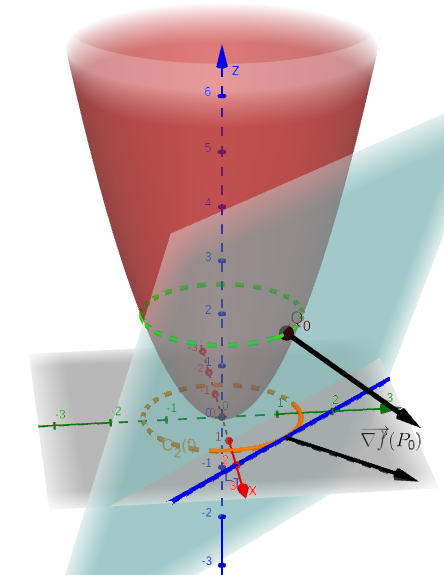
\includegraphics[scale=0.35]{img/ejercicios/3/1-a-5.png} 
\centering
\label{fig:1-a-5}
\end{figure}

\subsubsection*{3.1.a.6}
\label{subsubsec:3.1.a.6}
\addcontentsline{toc}{subsubsection}{\nameref{subsubsec:3.1.a.6}}

Observando la figura \ref{fig:1-a-5}, pueden verificarse las siguientes relaciones:

\begin{itemize}
\item El gradiente evaluado en $P_0$, vale decir $\overrightarrow{ \nabla f}(P_0)$ en el gráfico, es ortogonal al vector dirección de la recta tangente a la curva de nivel que pasa por $P_0$ ($C_2(f)$ en el dibujo) en el punto $P_0$.
\item El vector $N = (f_x(P_0), f_y(P_0), -1)$ es una normal válida del plano tangente a la superficie $z = f(x,y)$ en el punto $P_0$. Más específicamente, es la normal que apunta hacia el exterior de la superficie. Esto es consistente con el hecho de que el gradiente apunta en la dirección de mayor crecimiento de $f(x,y)$.
\end{itemize}

\subsection*{3.1.b}
\label{subsec:3.1.b}
\addcontentsline{toc}{subsection}{\nameref{subsec:3.1.b}}

\subsubsection*{3.1.b.1}
\label{subsubsec:3.1.b.1}
\addcontentsline{toc}{subsubsection}{\nameref{subsubsec:3.1.b.1}}

La función $f$ es $C^1$, con la salvedad de que al ser una raíz cuadrada, el radicando debe ser positivo. Por lo tanto, $\mathop{Dom}(f) = \{ (x,y) \in \Bbb R^2 / x^2 + y^2 \leq 4 \}$. Con eso en mente, el gradiente resulta:

\begin{align}
& \overrightarrow{ \nabla f }(x,y) = (f_x(x,y), f_y(x,y)) \\
& f_x(x,y) = \frac{\partial}{\partial x} [ (-x^2 -y^2 +4)^\frac{1}{2} ] = \frac{1}{2} (-x^2 -y^2 +4)^{-\frac{1}{2}} (-2x) = \frac{-x}{\sqrt{4-x^2-y^2}} \\
& f_y(x,y) = \frac{\partial}{\partial y} [ (-y^2 -x^2 +4)^\frac{1}{2} ] = \frac{-y}{\sqrt{4-x^2-y^2}}
\end{align}
 
Evaluando en $P_0 = (1,-1)$ resulta:

\begin{equation}
\overrightarrow{ \nabla f }(P_0) = \left( \frac{-1}{\sqrt{4-1-1}}, \frac{1}{\sqrt{4-1-1}} \right)
\end{equation}

\begin{equation}
\tcboxmath[colback=orange!25!white,colframe=orange,title=3.1.b.1]
{
\overrightarrow{ \nabla f }(P_0) = \left( -\frac{\sqrt{2}}{2}, \frac{\sqrt{2}}{2} \right)
}
\end{equation}

\subsubsection*{3.1.b.2}
\label{subsubsec:3.1.b.2}
\addcontentsline{toc}{subsubsection}{\nameref{subsubsec:3.1.b.2}}

La curva de nivel $k$ de $f$ es:

\begin{subequations}
\begin{align}
\mathop{Im}(f) &= [0,2] \Rightarrow \\
C_k(f) &= \{ (x,y) \in \Bbb R^2 / \sqrt{4-x^2-y^2} = k, k \in [0,2] \} \\
       &= \{ (x,y) \in \Bbb R^2 / x^2 + y^2 = 4-k^2, k \in [0, 2] \}
\end{align}
\end{subequations}

La curva asociada a $P_0$ corresponde a:

\begin{equation}
(1)^2 + (-1)^2 = 4-k^2 \Rightarrow 2 = 4-k^2 \Rightarrow 2 = k^2 \Rightarrow k = \sqrt{2}
\end{equation}

La solución $k=-\sqrt{2}$ no sirve en este caso porque $\mathop{Im}(f) = [0,2]$, lo cual excluye valores negativos de $k$. La curva de nivel buscada es entonces:

\begin{equation}
\tcboxmath[colback=orange!25!white,colframe=orange,title=3.1.b.2]
{
C_{\sqrt{2}}(f) = \{ (x,y) \in \Bbb R^2 / x^2 + y^2 = 2 \}
}
\end{equation}

Parametrizando para hallar la recta tangente en $P_0$:

\begin{subequations}
\begin{align}
& C_{\sqrt{2}}(f): \sigma(t) = (\sqrt{2} \cos(t), \sqrt{2} \sin(t)), t \in [0, 2\pi) \\
& \sigma'(t) = (-\sqrt{2} \sin(t), \sqrt{2} \cos(t)) \\
& \sigma(t_0) = P_0 \Rightarrow (\sqrt{2} \cos(t_0), \sqrt{2} \sin(t_0)) = (1, -1) \Rightarrow t_0 = \frac{7}{4} \pi \\
& \sigma'(t_0) = (1, 1)
\end{align}
\end{subequations}

La recta tangente en $P_0$ resulta entonces:

\begin{equation}
\tcboxmath[colback=orange!25!white,colframe=orange,title=3.1.b.2]
{
L_T: (1, 1) \alpha + (1, -1)
}
\end{equation}

Gráficamente, estos elementos pueden visualizarse en la figura \ref{fig:1-b-2}.

\begin{figure}[ht]
\caption{Curva de nivel, recta tangente y gradiente}
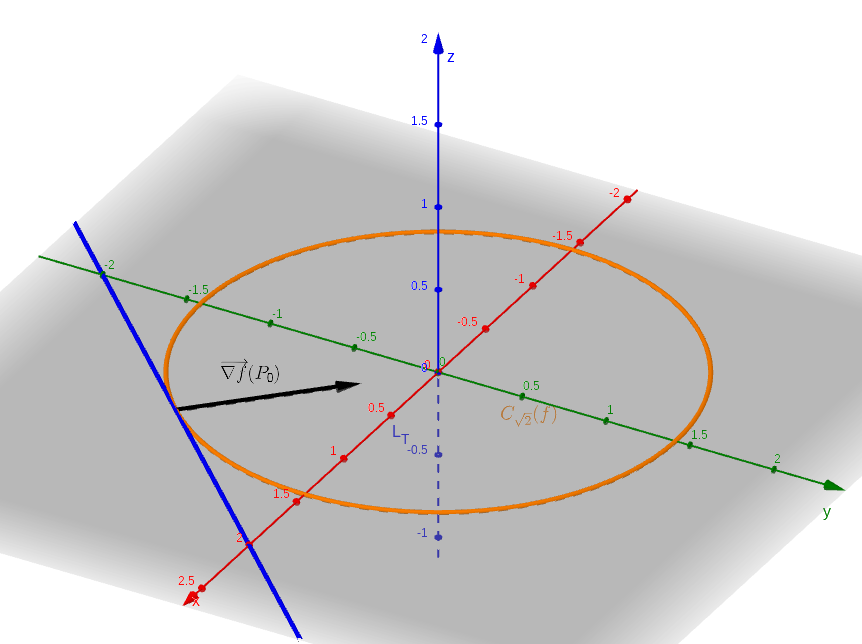
\includegraphics[scale=0.35]{img/ejercicios/3/1-b-2.png} 
\centering
\label{fig:1-b-2}
\end{figure}

\subsubsection*{3.1.b.3}
\label{subsubsec:3.1.b.3}
\addcontentsline{toc}{subsubsection}{\nameref{subsubsec:3.1.b.3}}

Primero, para calcular el plano tangente en un punto $P_0$, recúerdese que ello puede realizarse usando las derivadas parciales:

\begin{equation}
\Pi_T: z-z_0 - f_x(P_0) (x-x_0) - f_y(P_0) (y-y_0) = 0
\end{equation}

Para este caso, $x_0 = 1$, $y_0 = -1$, $z_0 = f(x_0,y_0) = \sqrt{4-1^2-(-1)^2} = \sqrt{2}$, $f_x(P_0) = -\frac{\sqrt{2}}{2}$, y $f_y(P_0) = \frac{\sqrt{2}}{2}$. Ergo:

\begin{subequations}
\begin{align}
& z-\sqrt{2} + \frac{\sqrt{2}}{2} (x-1) - \frac{\sqrt{2}}{2} (y+1) = 0 \\
& z-\sqrt{2} + \frac{\sqrt{2}}{2} x -\frac{\sqrt{2}}{2} -\frac{\sqrt{2}}{2}y -\frac{\sqrt{2}}{2} = 0 \\
& \frac{\sqrt{2}}{2} x -\frac{\sqrt{2}}{2} y + z - 2\sqrt{2} = 0 \\
& x -y + \sqrt{2} z -4 = 0
\end{align}
\end{subequations}

\begin{equation}
\tcboxmath[colback=orange!25!white,colframe=orange,title=3.1.b.3]
{
\Pi_T: x - y +\sqrt{2}z -4 = 0
}
\end{equation}

La superficie asociada a $z = \sqrt{4 - x^2 - y^2}$ puede analizarse en base a su imagen y curvas de nivel. La imagen es el intervalo $[0,2]$. Para $k = 0$, se tiene $0 = \sqrt{4 - x^2 - y^2} \Rightarrow x^2 + y^2 = 4$, o sea un círculo de radio 2. Para $k = 2$, se tiene $2 = \sqrt{4 - x^2 -y^2} \Rightarrow 4 = 4 -x^2-y^2 \Rightarrow x^2 + y^2 = 0$, o sea sólo el origen. En los valores intermedios, se tienen círculos con radio decreciente a medida que crece $z$. Ergo, la superficie tiene forma de cuenco invertido. El punto $Q_0$ no es otra cosa que $(x_0, y_0, f(x_0, y_0)) = (1, -1, \sqrt{2})$. Agregando la superficie y el plano tangente al gráfico previo, se obtiene la figura \ref{fig:1-b-3}.

\begin{figure}[ht]
\caption{Superficie y plano tangente}
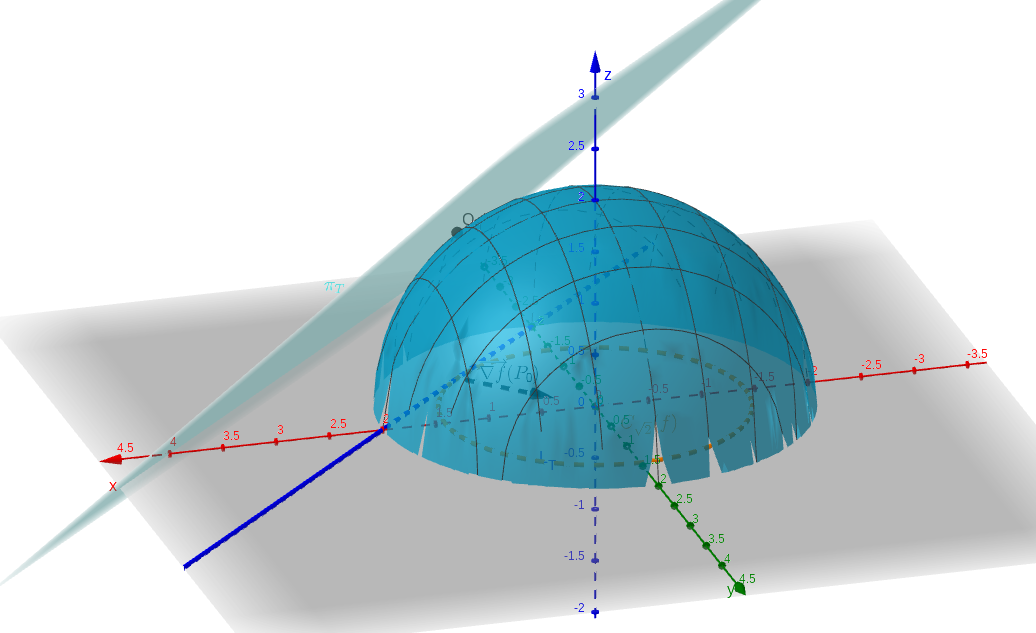
\includegraphics[scale=0.35]{img/ejercicios/3/1-b-3.png} 
\centering
\label{fig:1-b-3}
\end{figure}

\subsubsection*{3.1.b.4}
\label{subsubsec:3.1.b.4}
\addcontentsline{toc}{subsubsection}{\nameref{subsubsec:3.1.b.4}}

Recordando que las curvas de nivel pueden pensarse como cortes de la superficie a lo largo del eje $z$, la curva pedida es $C_{\sqrt{2}}(f)$, extendida a $\Bbb R^3$ fijando la componente $z = \sqrt{2}$. En otras palabras, es un círculo de radio $\sqrt{2}$ centrado en el origen del plano $z = \sqrt{2}$. Ello puede visualizarse en color morado en la figura \ref{fig:1-b-4}.

\begin{figure}[ht]
\caption{Curva de nivel en superficie}
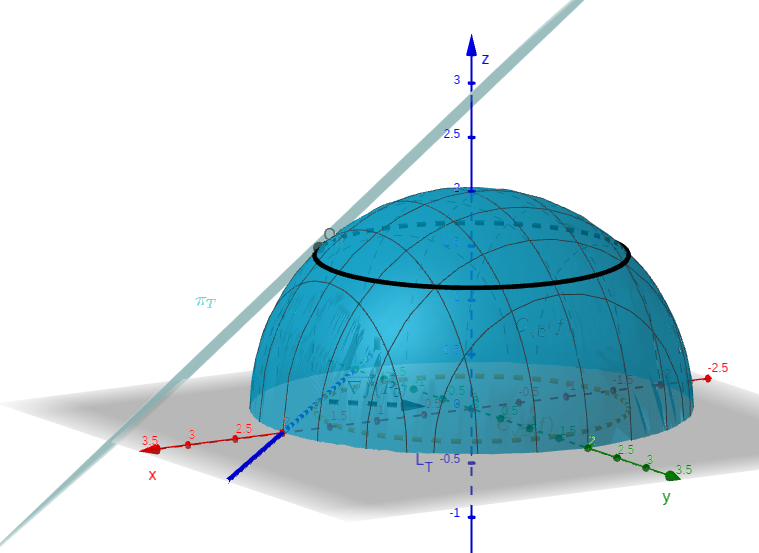
\includegraphics[scale=0.35]{img/ejercicios/3/1-b-4.png} 
\centering
\label{fig:1-b-4}
\end{figure}

\subsubsection*{3.1.b.5}
\label{subsubsec:3.1.b.5}
\addcontentsline{toc}{subsubsection}{\nameref{subsubsec:3.1.b.5}}

El valor de $N$ es:

\begin{equation}
N = (fx(x_0,y_0), f_y(x_0,y_0), -1) = \left( -\frac{\sqrt{2}}{2}, \frac{\sqrt{2}}{2}, -1 \right)
\end{equation}

Graficando $N$ con origen en $Q_0$, se obtiene el vector negro de la figura \ref{fig:1-b-5}.

\begin{figure}[ht]
\caption{Vector normal a la superficie}
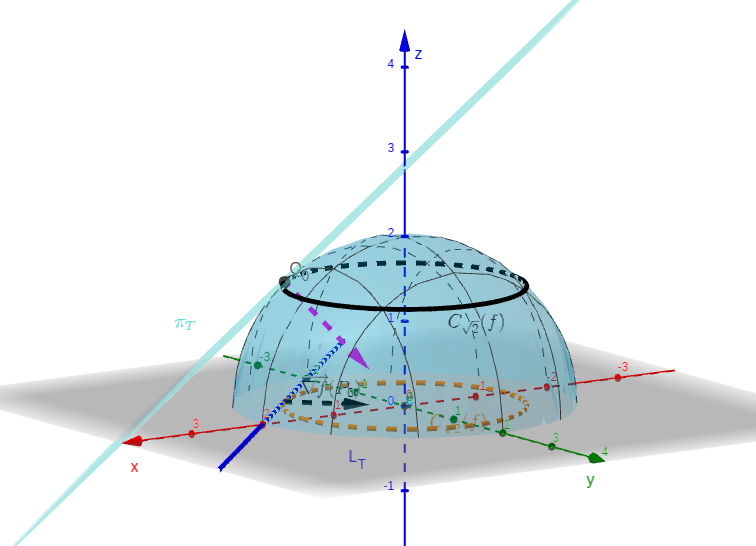
\includegraphics[scale=0.35]{img/ejercicios/3/1-b-5.png} 
\centering
\label{fig:1-b-5}
\end{figure}

\subsubsection*{3.1.b.6}
\label{subsubsec:3.1.b.6}
\addcontentsline{toc}{subsubsection}{\nameref{subsubsec:3.1.b.6}}

Observando la figura \ref{fig:1-b-5}, pueden verificarse las siguientes relaciones:

\begin{itemize}
\item El gradiente evaluado en $P_0$, vale decir $\overrightarrow{ \nabla f}(P_0)$ en el gráfico, es ortogonal al vector dirección de la recta tangente a la curva de nivel que pasa por $P_0$ ($C_{\sqrt{2}}(f)$ en el dibujo) en el punto $P_0$.
\item El vector $N = (f_x(P_0), f_y(P_0), -1)$ es una normal válida del plano tangente a la superficie $z = f(x,y)$ en el punto $P_0$. Más específicamente, es la normal que apunta hacia el interior de la superficie. Esto es consistente con el hecho de que el gradiente apunta en la dirección de mayor crecimiento de $f(x,y)$. En el ejercicio anterior, la normal apuntaba hacia afuera, y ahora hacia adentro; esto parecería una inconsistencia, pero tiene sentido si se piensa que el gradiente apunta en la dirección de máximo crecimiento del valor escalar $z = f(x,y)$. En el caso anterior, al crecer $x$ e $y$, crece $z$, por ello el gradiente apunta hacia afuera de la superficie. En el caso del ejercicio actual, el valor de $z$ crece al acercarse al origen, ya que allí está su valor máximo. Por eso el gradiente apunta hacia el origen, y $N$ pasa a apuntar hacia el interior de la superficie.
\end{itemize}

\subsection*{3.1.c}
\label{subsec:3.1.c}
\addcontentsline{toc}{subsection}{\nameref{subsec:3.1.c}}

\subsubsection*{3.1.c.1}
\label{subsubsec:3.1.c.1}
\addcontentsline{toc}{subsubsection}{\nameref{subsubsec:3.1.c.1}}

Por simple inspección, $f \in C^1(\Bbb R^2)$. El gradiente resulta:

\begin{align}
& \overrightarrow{ \nabla f }(x,y) = (f_x(x,y), f_y(x,y)) = \left( \frac{\partial}{\partial x}(5 +2x -3y), \frac{\partial}{\partial y}(5 +2x -3y) \right) = (2,-3)
\end{align}
 
El gradiente es entonces constante:

\begin{equation}
\tcboxmath[colback=orange!25!white,colframe=orange,title=3.1.c.1]
{
\overrightarrow{ \nabla f }(P_0) = (2, -3)
}
\end{equation}

\subsubsection*{3.1.c.2}
\label{subsubsec:3.1.c.2}
\addcontentsline{toc}{subsubsection}{\nameref{subsubsec:3.1.c.2}}

La curva de nivel $k$ de $f$ es:

\begin{subequations}
\begin{align}
\mathop{Im}(f) &= \Bbb R \Rightarrow \\
C_k(f) &= \{ (x,y) \in \Bbb R^2 / 5 +2x -3y = k, k \in \Bbb R \} \\
       &= \left\{ (x,y) \in \Bbb R^2 / y = \frac{2}{3} x + \frac{5-k}{3}, k \in \Bbb R \right\}
\end{align}
\end{subequations}

La curva asociada a $P_0$ corresponde a:

\begin{equation}
5 + 2 \cdot 0 - 3 \cdot 0 = k \Rightarrow k = 5
\end{equation}

La curva de nivel buscada es entonces:

\begin{equation}
\tcboxmath[colback=orange!25!white,colframe=orange,title=3.1.c.2]
{
C_{5}(f) = \left\{ (x,y) \in \Bbb R^2 / y = \frac{2}{3} x \right\}
}
\end{equation}

Parametrizando para hallar la recta tangente en $P_0$:

\begin{subequations}
\begin{align}
& C_{5}(f): \sigma(t) = \left( t, \frac{2}{3}t \right), t \in \Bbb R \\
& \sigma'(t) = \left( 1, \frac{2}{3} \right)
\end{align}
\end{subequations}

La recta tangente en $P_0$ resulta entonces:

\begin{equation}
\tcboxmath[colback=orange!25!white,colframe=orange,title=3.1.c.2]
{
L_T: \left( 1, \frac{2}{3} \right) \alpha
}
\end{equation}

Gráficamente, estos elementos pueden visualizarse en la figura \ref{fig:1-c-2}.

\begin{figure}[ht]
\caption{Curva de nivel, recta tangente y gradiente}
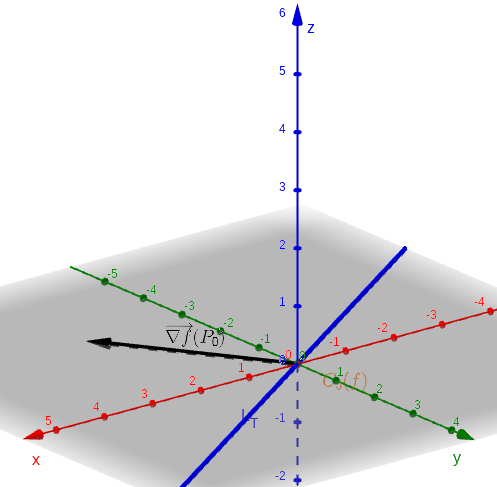
\includegraphics[scale=0.35]{img/ejercicios/3/1-c-2.png} 
\centering
\label{fig:1-c-2}
\end{figure}

Nótese que la curva de nivel es una recta; por lo tanto, en todo punto, la tangente coincide con ella misma.

\subsubsection*{3.1.c.3}
\label{subsubsec:3.1.c.3}
\addcontentsline{toc}{subsubsection}{\nameref{subsubsec:3.1.c.3}}

Primero, para calcular el plano tangente en un punto $P_0$, recúerdese que ello puede realizarse usando las derivadas parciales:

\begin{equation}
\Pi_T: z-z_0 - f_x(P_0) (x-x_0) - f_y(P_0) (y-y_0) = 0
\end{equation}

Para este caso, $x_0 = 0$, $y_0 = 0$, $z_0 = f(x_0,y_0) = 5$, $f_x(P_0) = 2$, y $f_y(P_0) = -3$. Ergo:

\begin{subequations}
\begin{align}
& z-5 - 2 (x-0) + 3 (y-0) = 0 \\
& z-5 -2x +3y = 0 \\
& -2x +3y -z +5 = 0
\end{align}
\end{subequations}

\begin{equation}
\tcboxmath[colback=orange!25!white,colframe=orange,title=3.1.c.3]
{
\Pi_T: 2x -3y -z +5 = 0
}
\end{equation}

La superficie asociada a $z = 2x -3y +5$, que es un plano que coincide punto a punto con el plano tangente. El punto $Q_0$ es $(x_0, y_0, f(x_0,y_0)) = (0,0,5)$ Agregando la superficie, el plano tangente y el punto $Q_0$ al gráfico previo, se obtiene la figura \ref{fig:1-c-3}.

\begin{figure}[ht]
\caption{Superficie y plano tangente}
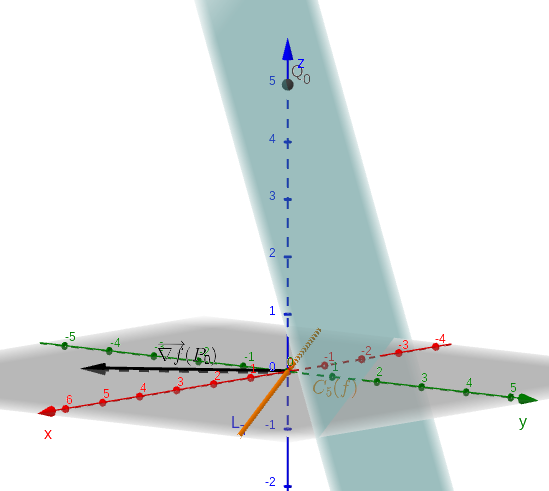
\includegraphics[scale=0.35]{img/ejercicios/3/1-c-3.png} 
\centering
\label{fig:1-c-3}
\end{figure}

\subsubsection*{3.1.c.4}
\label{subsubsec:3.1.c.4}
\addcontentsline{toc}{subsubsection}{\nameref{subsubsec:3.1.c.4}}

Recordando que las curvas de nivel pueden pensarse como cortes de la superficie a lo largo del eje $z$, la curva pedida es $C_{5}(f)$, extendida a $\Bbb R^3$ fijando la componente $z = 5$. En otras palabras, es la recta $y = \frac{2}{3}x$ centrada en el origen del plano $z = 5$. Ello puede visualizarse en color negro en la figura \ref{fig:1-c-4}.

\begin{figure}[ht]
\caption{Curva de nivel en superficie}
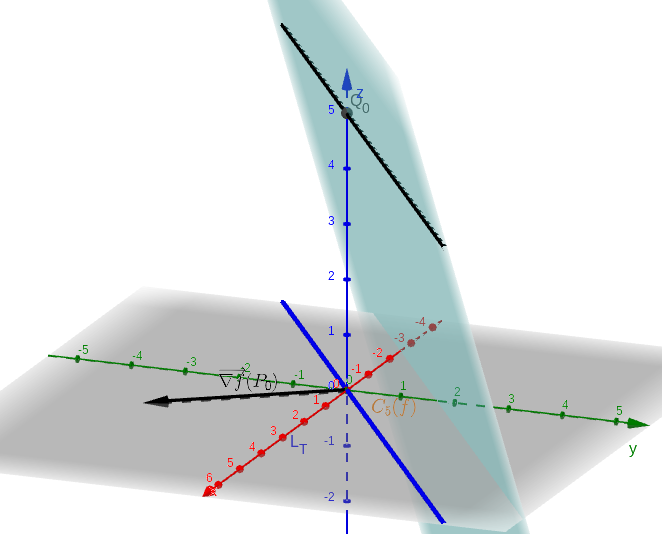
\includegraphics[scale=0.35]{img/ejercicios/3/1-c-4.png} 
\centering
\label{fig:1-c-4}
\end{figure}

\subsubsection*{3.1.c.5}
\label{subsubsec:3.1.c.5}
\addcontentsline{toc}{subsubsection}{\nameref{subsubsec:3.1.c.5}}

El valor de $N$ es:

\begin{equation}
N = (fx(x_0,y_0), f_y(x_0,y_0), -1) = (2, -3, -1)
\end{equation}

Graficando $N$ con origen en $Q_0$, se obtiene el vector rosa de la figura \ref{fig:1-c-5}.

\begin{figure}[ht]
\caption{Vector normal a la superficie}
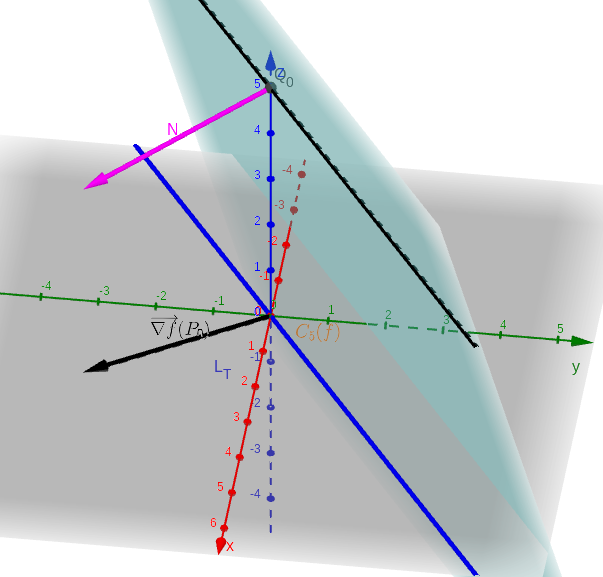
\includegraphics[scale=0.35]{img/ejercicios/3/1-c-5.png} 
\centering
\label{fig:1-c-5}
\end{figure}

\subsubsection*{3.1.c.6}
\label{subsubsec:3.1.c.6}
\addcontentsline{toc}{subsubsection}{\nameref{subsubsec:3.1.c.6}}

Observando la figura \ref{fig:1-c-5}, pueden verificarse las siguientes relaciones:

\begin{itemize}
\item El gradiente evaluado en $P_0$, vale decir $\overrightarrow{ \nabla f}(P_0)$ en el gráfico, es ortogonal al vector dirección de la recta tangente a la curva de nivel que pasa por $P_0$ ($C_{\sqrt{2}}(f)$ en el dibujo) en el punto $P_0$.
\item El vector $N = (f_x(P_0), f_y(P_0), -1)$ es una normal válida del plano tangente a la superficie $z = f(x,y)$ en el punto $P_0$. En este caso, superficie y plano tangente coinciden: la superficie es un plano y por ende no es cerrada, por lo cual no puede hablarse de interior o exterior. Sin embargo, el gradiente sigue apuntando en la dirección de mayor crecimiento de $z$: valores positivos de $x$ y valores negativos de $y$ (por el coeficiente $-3$): en dicha dirección, $z$ crece hacia $+\infty$.
\end{itemize}

\subsection*{3.1.d}
\label{subsec:3.1.d}
\addcontentsline{toc}{subsection}{\nameref{subsec:3.1.d}}

\subsubsection*{3.1.d.1}
\label{subsubsec:3.1.d.1}
\addcontentsline{toc}{subsubsection}{\nameref{subsubsec:3.1.d.1}}

Por simple inspección, $f \in C^1(\Bbb R^2)$. El gradiente resulta:

\begin{align}
& \overrightarrow{ \nabla f }(x,y) = (f_x(x,y), f_y(x,y)) = \left( \frac{\partial}{\partial x}(7 +x y), \frac{\partial}{\partial y}(7 + xy) \right) = (y, x)
\end{align}
 
Evaluando el gradiente en $P_0 = (0,0)$ se obtiene entonces:

\begin{equation}
\tcboxmath[colback=orange!25!white,colframe=orange,title=3.1.d.1]
{
\overrightarrow{ \nabla f }(P_0) = (0, 0)
}
\end{equation}

\end{document}
